\documentclass[conference]{IEEEtran}
\IEEEoverridecommandlockouts
% The preceding line is only needed to identify funding in the first footnote. If that is unneeded, please comment it out.
\usepackage{cite}
\usepackage{amsmath,amssymb,amsfonts}
\usepackage{algorithmic}
\usepackage{graphicx}
\usepackage{textcomp}
\usepackage{xcolor}
\usepackage{booktabs}
\def\BibTeX{{\rm B\kern-.05em{\sc i\kern-.025em b}\kern-.08em
    T\kern-.1667em\lower.7ex\hbox{E}\kern-.125emX}}
\begin{document}

\title{Miniproject 1 - Machine Learning 101 \\
{\small COMP551 - Applied Machine Learning}
}

\author{\IEEEauthorblockN{Ege Odaci}
\IEEEauthorblockA{\textit{McGill University} \\
ege.odaci@mail.mcgill.ca}
\and
\IEEEauthorblockN{Rafael Gomes Braga}
\IEEEauthorblockA{\textit{École de Thechnologie Supérieure} \\
rafael.gomes-braga.1@ens.etsmtl.ca}
\and
\IEEEauthorblockN{Ramon Figueiredo Pessoa}
\IEEEauthorblockA{\textit{École de Thechnologie Supérieure} \\
ramon.figueiredo-pessoa.1@ens.etsmtl.ca}
}

\maketitle

\begin{abstract}
 In this mini-project we studied the performance of two classification models, namely Logistic Regression (LR) and Naive Bayes(NB), on four benchmark datasets. We analysed the features and labels of each dataset and applied preprocessing techniques to prepare the data to be used with the learning algorithms. We then performed some experiments to learn how the models behave in relation to each dataset. For both models we evaluated their performance with different sizes of training sets and for Logistic Regression we tried different values for the learning rate. After finding the best values for those parameters, we used 5-fold cross validation and choose the best performing models. We learned that both models performed comparably for all datasets, except for the Wine Quality one, in which Logistic Regression performed poorly. Finally, we compared our implementations to the corresponding ones provided by the scikit-learn package.
\end{abstract}


\section{Introduction}

In this first project we experimented on the performance of the two significant classification models Logistic Regression and Naive Bayes on all four datasets. To begin with each dataset was analyzed to see what kind a information is stored in them. Ionosphere data was collected in Gose Bay, Labrador using 16 high frequency antennas and reported the signals and a label classifying these signals as b for bad and g for good. As can be seen from ionosphere.name file, even indexed columns are used to store the real values whereas the odd indexed columns are used to store complex values thus there is no correlation between them. First column consists of many 1's in contrast to second column being filled with many 0's.    \cite{ionosphere} Adult data involves some non continuous information such as working class, education, marital status, occupation, relationship, race, sex and native country recorded as strings. Adult data also involves some continuous information which are age, total education in years, capital gain, capital loss, hours per week and final weight recorded as integers \cite{adult}. At the very last column it specifies for each person whether they make more or less than 50K US dollars. Our third dataset is about breast cancer cells which collected from University of Wisconsin Hospitals. Each record have id number and some important attributes rated between 1 to 10. At the last column it specifies the cancer cell as 2 for Benign or 4 for Malignant \cite{cancer}. Final dataset is about Wine Quality, It has scientific information stored as floats about the ingredients of the wine such as pH, fixed acidity etc. Last column stores the general rating for each wine, calculated by the median of at least 3 wine expert's rating \cite{wine}. Logistic Regression and Naive Bayes are tested on each dataset with different training sizes then their accuracies were compared to each other. For Ionosphere dataset both Logical Regression and Naive Bayes outputted nice accuracy with Logical Regression having slightly higher accuracy. For the adult dataset we observed that Logical Regression has provided better accuracy. With Wine dataset, Naive Bayes has given significantly high accuracy. For the breast cancer dataset, both models have really high accuracy with Logical Regression having higher accuracy.



\section{Datasets}
\label{section:datasets}

\subsection{Output Labels}

Since we are studying binary classification tasks, we needed to be sure that each dataset only outputs two possible labels. This is true for all datasets, except the Wine Quality one, which outputs a number from 1 to 10. We converted that dataset to a binary task by changing its output to 0 where the original value was less than or equal to 5 and 1 otherwise. We also computed the distributions of the two classes for each dataset and summarize it in Figure \ref{fig:output_labels}.

\begin{figure}%
\centering
\subfigure[a]{%
\label{fig:ex3-a}%
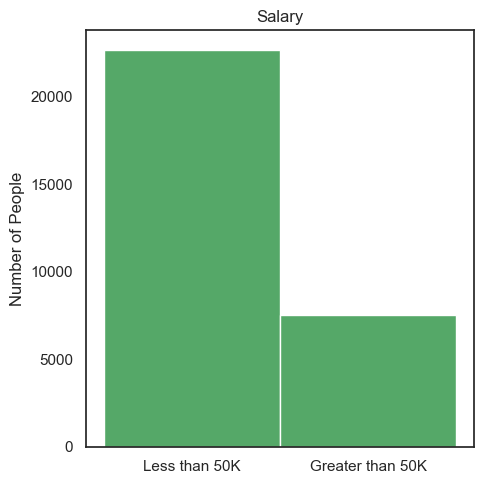
\includegraphics[scale = 0.39]{figs/histograms/ADULT.png}}%
\hspace{8pt}%
\subfigure[b]{%
\label{fig:ex3-b}%
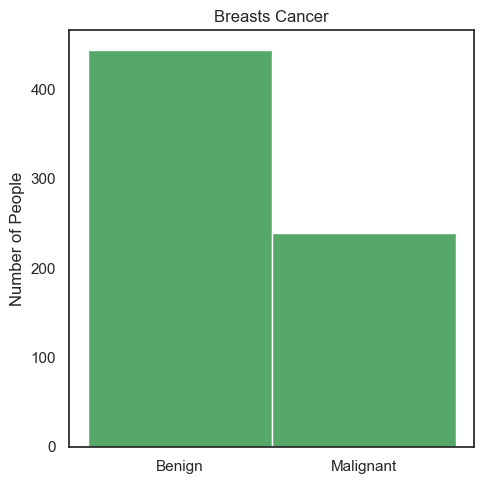
\includegraphics[scale = 0.39]{figs/histograms/BREAST_CANCER_DIAGNOSIS.png}} \\
\subfigure[c]{%
\label{fig:ex3-c}%
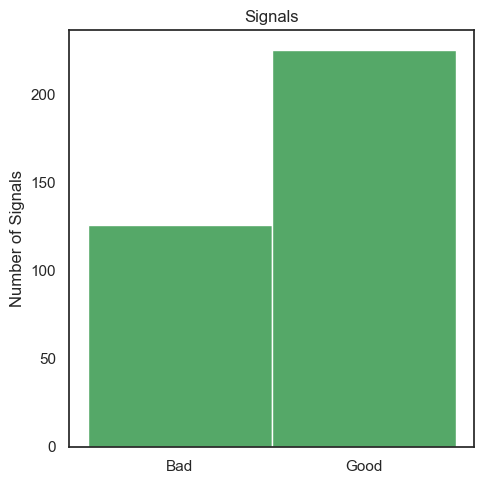
\includegraphics[scale = 0.39]{figs/histograms/IONOSPHERE.png}}%
\hspace{8pt}%
\subfigure[d]{%
\label{fig:ex3-d}%
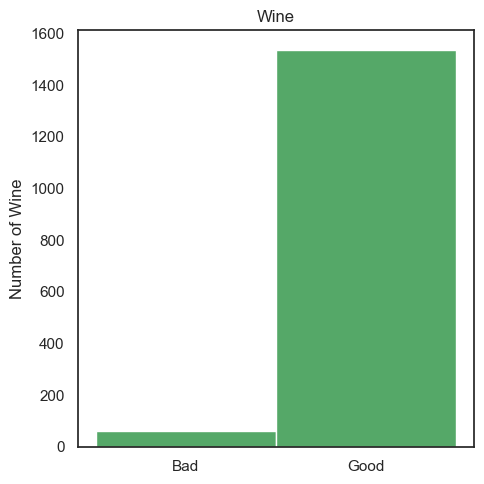
\includegraphics[scale = 0.39]{figs/histograms/WINE_QUALITY.png}}%
\caption[Distributions of the positive vs.
negative classes (histogram).]{Distributions of the positive vs.
negative classes (histogram):
\subref{a} Adult;
\subref{b} Breast Cancer Diagnosis;
\subref{c} Ionosphere; and,
\subref{d} Wine Quality.}%
\label{fig:output_labels}%
\end{figure}

\subsection{Missing Data and Malformed Features}

The Adult and Breast Cancer Diagnosis datasets have points with missing values for some of the features, represented by the '?' symbol. We decided to remove those points. We also found some malformed features and irrelevant features:

\begin{itemize}
    \item In the Ionosphere dataset 89.2\% of the values of the first feature and all the values of the second feature are zero
    \item In the Adult dataset the columns labeled "capital-gain" and "capital-loss" are also mostly composed of zeros (91.7\% and 95.3\% respectively)
    \item The first feature of the Breast Cancer dataset is the sample code number, which has no influence if the cancer is benign or malignant
\end{itemize}

We decided to remove those features completely.

\subsection{Continuous Fetures}

All features in the Ionosphere, Breast Cancer Diagnosis and Wine Quality datasets and 6 features in the Adult dataset are continuous. We plotted histograms and computed basic statistics for each of them in order to understand their distribution. We also applied stardardization to make the so the data has similar scales.

\subsetion{Categorical Features}

The Adult dataset have 8 categorical features. We applied one-hot encoding to convert those values to numeric.

\subsection{Correlation between features}

We draw heatmaps of feature versus feature to understand how they are correlated to each other. We found out that some of the features are highly correlated with other ones. Figure \ref{fig:heatmap} shows some of the more interesting heatmaps.

\begin{figure}%
\label{fig:heatmap}%
\centering
\subfigure[a]{%
\label{fig:ex3-a}%
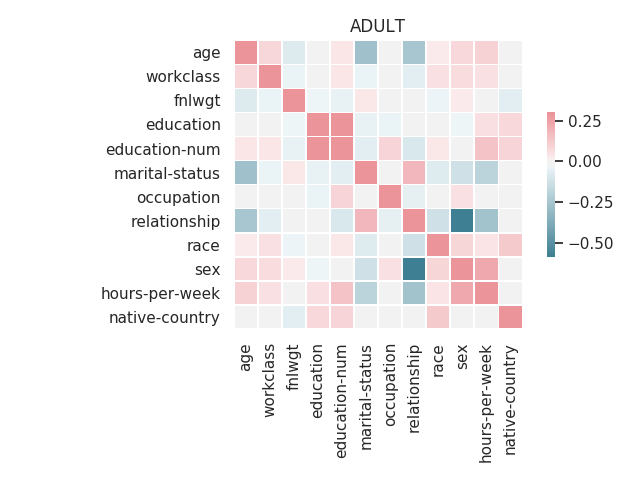
\includegraphics[scale = 0.39]{figs/heatmaps/ADULT.png}}%
\hspace{8pt}%
\subfigure[b]{%
\label{fig:ex3-b}%
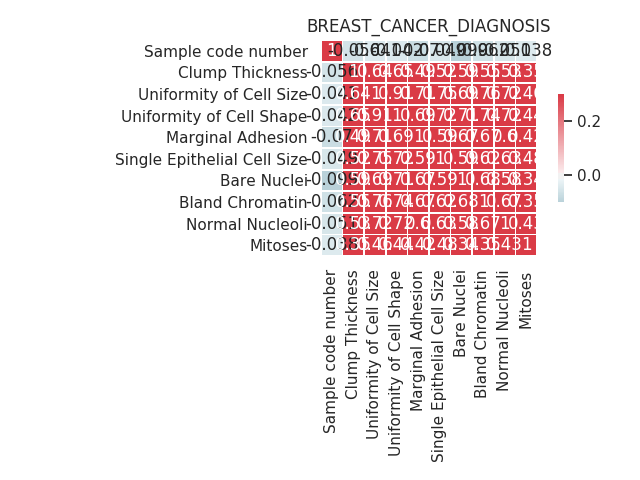
\includegraphics[scale = 0.39]{figs/heatmaps/BREAST_CANCER_DIAGNOSIS.png}} \\
\subfigure[c]{%
\label{fig:ex3-c}%
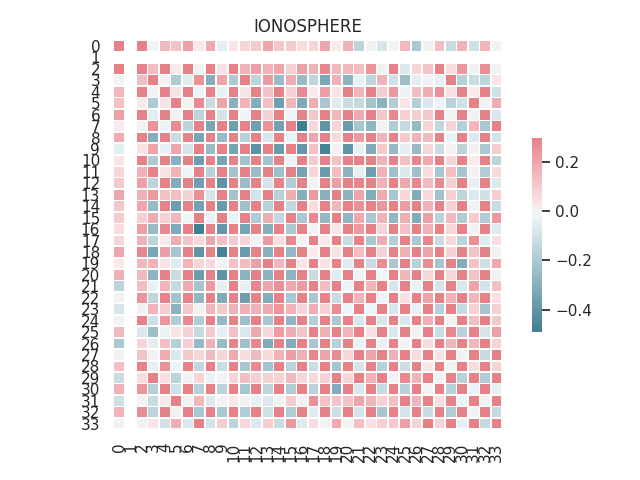
\includegraphics[scale = 0.39]{figs/heatmaps/IONOSPHERE.png}}%
\hspace{8pt}%
\subfigure[d]{%
\label{fig:ex3-d}%
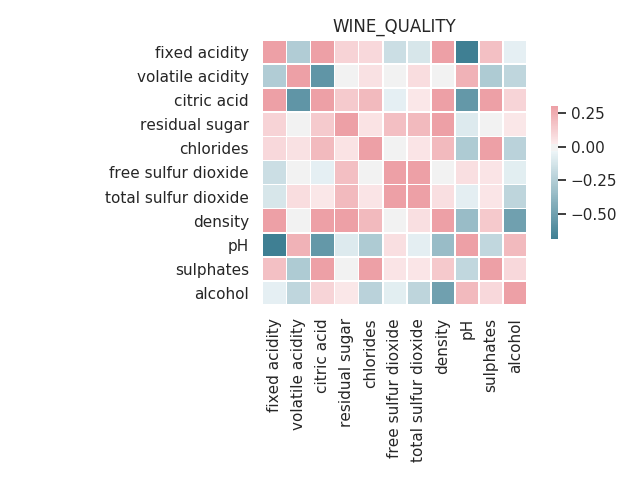
\includegraphics[scale = 0.39]{figs/heatmaps/WINE_QUALITY.png}}%
\caption[Dataset heatmaps (correlation matrix).]{Dataset heatmaps (correlation matrix):
\subref{a} Adult;
\subref{b} Breast Cancer Diagnosis;
\subref{c} Ionosphere; and,
\subref{d} Wine Quality.}%
\end{figure}

\section{Results}
\label{section:results}

\subsection{Testing Different Training Sizes}

In this experiment we trained our models against all datasets varying the size of the trainning data from 5\% to 95\%, and computed the accuracy of the prediction for each case. Figure \ref{fig:ex3} shows the results.

\begin{figure}%
\centering
\subfigure[a]{%
\label{fig:ex3-a}%
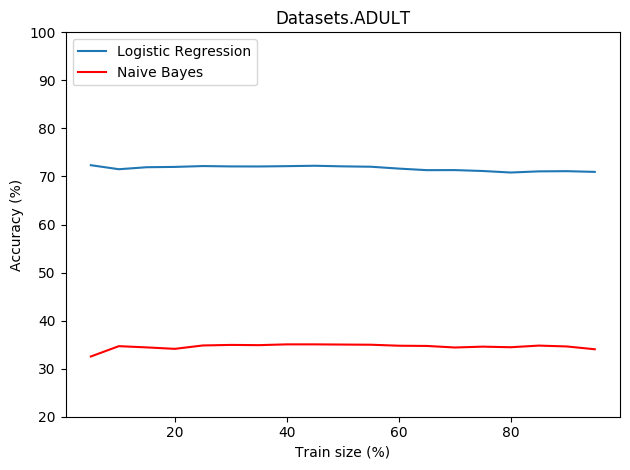
\includegraphics[scale = 0.39]{figs/accuracy_vs_trainingsize/DatasetsADULT.png}}%
\hspace{8pt}%
\subfigure[b]{%
\label{fig:ex3-b}%
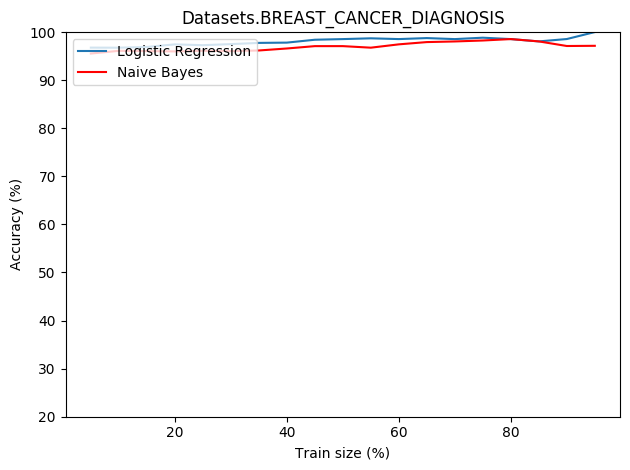
\includegraphics[scale = 0.39]{figs/accuracy_vs_trainingsize/DatasetsBREAST_CANCER_DIAGNOSIS.png}} \\
\subfigure[c]{%
\label{fig:ex3-c}%
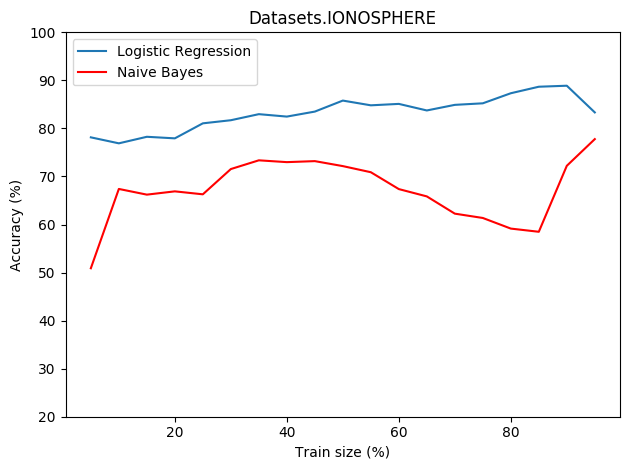
\includegraphics[scale = 0.39]{figs/accuracy_vs_trainingsize/DatasetsIONOSPHERE.png}}%
\hspace{8pt}%
\subfigure[d]{%
\label{fig:ex3-d}%
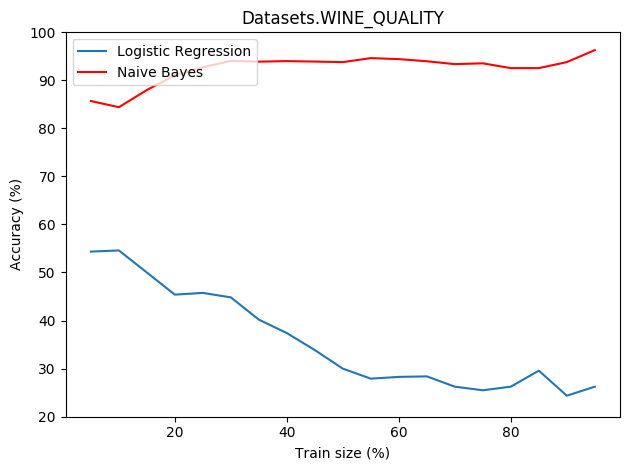
\includegraphics[scale = 0.39]{figs/accuracy_vs_trainingsize/DatasetsWINE_QUALITY.png}}%
\caption[Comparing the accuracy of the two models (LR and NB) as a function of the size of the training set]{Comparing the accuracy of the two models (LR and NB) as a function of the size of the training set):
\subref{a} Adult;
\subref{b} Breast Cancer Diagnosis;
\subref{c} Ionosphere; and,
\subref{d} Wine Quality.}%
\label{fig:ex3}%
\end{figure}

We observe that for some of the datasets the accuracy varies a lot as the function of the training size, while for others it is almost constant. We also tried shuffling the data before splitting it into training and testings sets. Figure \ref{fig:data_size_shufle} shows the results obtained after shuffling.

\begin{figure}%
\centering
\subfigure[a]{%
\label{fig:ex3-a}%
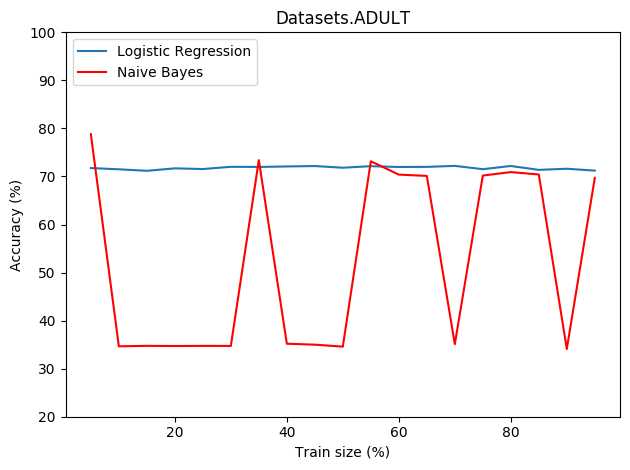
\includegraphics[scale = 0.39]{figs/accuracy_vs_trainingsize/DatasetsADULT_shuffle.png}}%
\hspace{8pt}%
\subfigure[b]{%
\label{fig:ex3-b}%
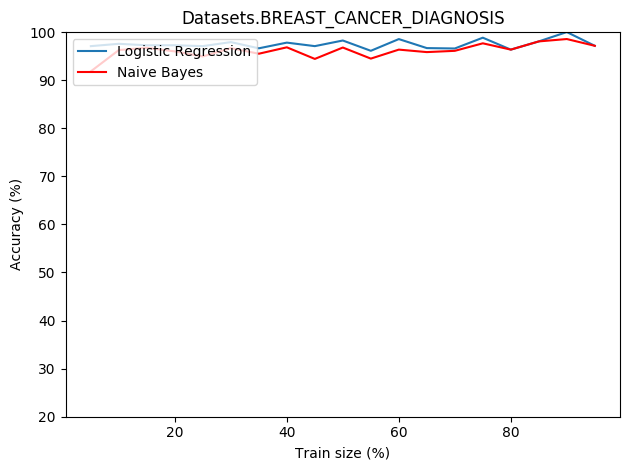
\includegraphics[scale = 0.39]{figs/accuracy_vs_trainingsize/DatasetsBREAST_CANCER_DIAGNOSIS_shuffle.png}} \\
\subfigure[c]{%
\label{fig:ex3-c}%
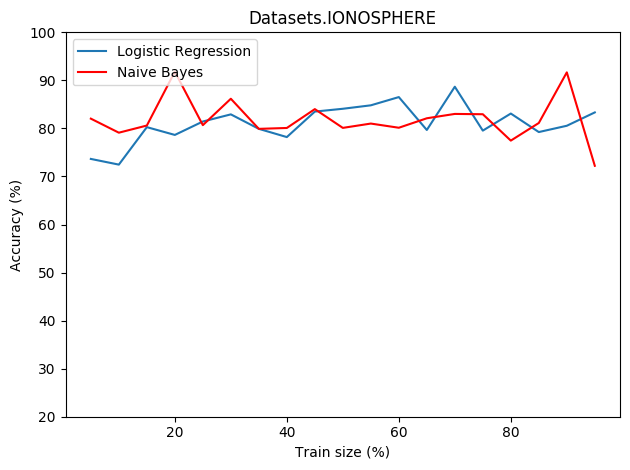
\includegraphics[scale = 0.39]{figs/accuracy_vs_trainingsize/DatasetsIONOSPHERE_shuffle.png}}%
\hspace{8pt}%
\subfigure[d]{%
\label{fig:ex3-d}%
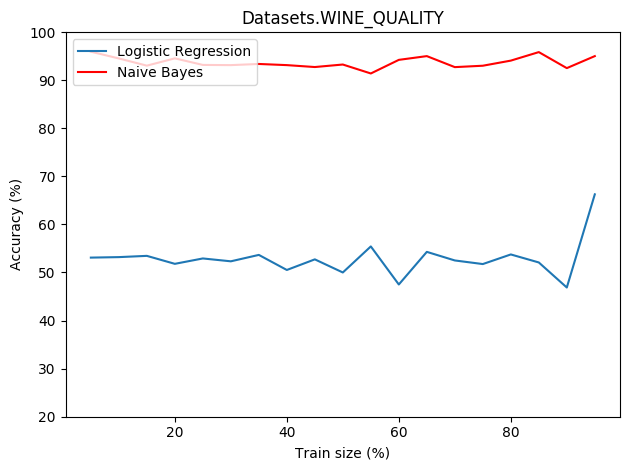
\includegraphics[scale = 0.39]{figs/accuracy_vs_trainingsize/DatasetsWINE_QUALITY_shuffle.png}}%
\caption[Comparing the accuracy as a function of training size with shuffling]{Comparing the accuracy as a function of training size with shuffling:
\subref{a} Adult;
\subref{b} Breast Cancer Diagnosis;
\subref{c} Ionosphere; and,
\subref{d} Wine Quality.}%
\label{fig:ex3}%
\end{figure}

We observe that shuffling actually increased the overall accuracy of the models. Based on this result, we choose to use the value 80\% for the splitting, with shuffling.

\subsection{Different Values of Learning Rate for Logistic Regression}

In this test we ran Logistic Regression against all datasets varying the learning rate to understand which value would give us the fastest training time. Image \ref{fig:learning_rate} shows a plot of the cost function against number of iterations for varying learning rates against the Adult dataset. The plots for the other datasets have a similar format.

\begin{figure}
\label{fig:learning_rate}
\centering
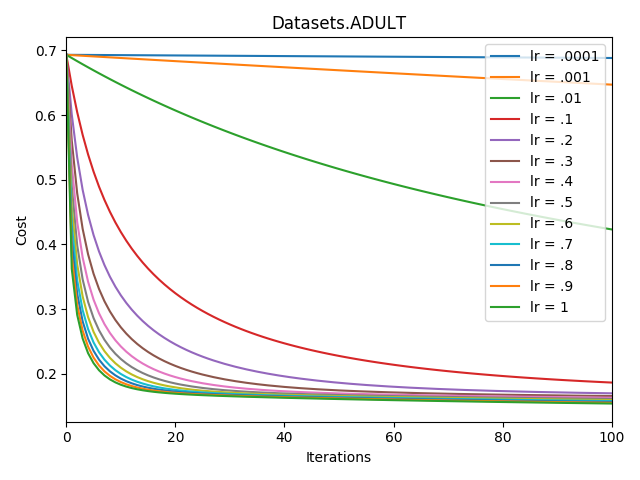
\includegraphics[scale = 0.39]{figs/cost_vs_iterations/ADULT.png}
\caption[Cost function versus number of iterations for Logistic Regression against the Adult dataset for different learning rates]{Cost function versus number of iterations for Logistic Regression against the Adult dataset for different learning rates}
\end{figure}

Here we noticed that, as expected, increasing the learning rate increases the speed of the training process. We decided to use the value of 1 for our next tests since it makes the cost function converge very fast.


\subsection{Comparison between Logistic Regression and Naive Bayes}

After selecting the best parameters we trained the Logistic Regression and Naive Bayes models against all datasets to compare their performances. We also wanted to compare our implementation to industry standard ones so we imported the scikit-learn and used their implementation of the two algorithms on the same datasets. Table \ref{table:accuracy} summarizes the results for all runs we did.

\begin{table}
  \caption{Testing accuracy of Linear Regression (LR) and Naive Bayes (NB) versus the corresponding scikit-learn implementations (SK-LR and SK-NB) for each of the four datasets}
  \label{table:accuracy}
  \centering
  \begin{tabular}{lllll}
    \toprule
    Dataset       & LR   & NB   & SK-LR & SK-NB \\
    \midrule
    Ionosphere    & 83.09\% & 85.91\% & 81.69\% & 76.05\%  \\
    Adult         & 71.92\% & 72.66\% & 82.06\% & 75.21\%  \\
    Wine Quality  & 56.25\% & 95.31\% & 96.56\% & 94.06\%  \\
    Breast Cancer & 96.35\% & 97.08\% & 96.35\% & 97.08\%  \\
    \bottomrule
  \end{tabular}
\end{table}

Here we can see that our Naive Bayes implementation obtained results comparable to the scikit-learn implementation for all datasets. The Naive Bayes model, however, obtained bad results agains the Wine Quality dataset.

We also implemented and applied cross validation and summarize the results in Table \ref{table:cross}.

\begin{table}
  \caption{K-fold cross validation (k=5) scores: of Linear Regression (LR) and Naive Bayes (NB) versus the corresponding scikit-learn implementations (SK-LR and SK-NB) for each of the four datasets}
  \label{table:cross}
  \centering
  \begin{tabular}{lllll}
    \toprule
    Dataset       & Scores (\%): K-fold cross validation (k=5) \\
    \midrule
    LR: Ionosphere    & [80.35, 83.92, 82.14, 80.35, 85.71]  \\
    LR: Adult         & [71.93, 71.82, 71.59, 71,47, 71.55]  \\
    LR: Wine & [48.04, 49.60, 50, 51.17, 57.64]  \\
    LR: Cancer & [94.54, 98.16, 97.24, 97.24, 98.16]  \\
    
    SK-LR: Ionosphere    & [87.50, 87.50, 76.78, 87.50 , 87.50]  \\
    SK-LR: Adult         & [81.88, 82.11, 81.85, 82.70, 82.57]  \\
    SK-LR: Wine  & [96.48, 96.09, 95.70, 94.53, 97.25]  \\
    SK-LR: Cancer & [96.36, 97.24, 95.41, 95.41, 97.24]  \\
    
    NB: Ionosphere    & [75.00, 92.85, 83.92, 83.92, 73.21]  \\
    NB: Adult         & [36.30, 36.06, 37.77, 34.81, 37.00]  \\
    NB: Wine  & [94.53, 92.18, 94.14, 93.35, 92.54 ]  \\
    NB: Cancer & [92.72, 97.24, 97.24, 95.41, 98.16] \\
    
    SK-NB: Ionosphere    & [82.14, 87.50, 73.21, 91.07, 75.00] \\
    SK-NB: Adult         & [69.81, 70.42, 70.76, 34.18, 71.27]  \\
    SK-NB: Wine & [92.57, 94.53, 96.87, 93.75, 92.94]  \\
    SK-NB: Cancer & [95.45, 96.33, 94.49, 96.33, 98.16]  \\
    \bottomrule
  \end{tabular}
\end{table}

\section{Discussion and Conclusion}
\label{section:discussion}

After performing all the experiments, we were able to improve our models obtaining good results against all datasets, except for one case: Logistic Regression against the Wine Quality dataset. Unfortunately we didn't have enough time to investigate further why that was happening. However, we used a similar implementation with the scikit-learn package to compare to algorithms and observed that the performances were comparable. We learned that one of the most important steps is the data analysis and preprocessing. For the future, it would be interesting to work again with the Wine dataset using its output column original value, treating it as a multiclass problem. 

\section{Statement of Contributions}
\label{section:contributions}

Ege worked on the visualization and analysis of the datasets, and implemented the \textit{evaluate\_acc} function. Rafael implemented the machine learning models and performed the experiments. Ramon worked on the preprocessing of data, provided the \textit{sklearn} implementation that we used as benchmark,  developed the k-fold cross validation script and created the command line interface.

\medskip

\small

\begin{thebibliography}{9}
\bibitem{ionosphere} 
V. G. Sigillito, S. P. Wing, L. V. Hutton, and K. B.
Baker 
\textit{ “Classification of radar returns from the
ionosphere using neural networks,”} 
 Johns Hopkins APL Tech. Dig. Applied Phys. Lab., 1989. 
 
 \bibitem{adult} 
Ron Kohavi
\textit{ “Scaling Up the Accuracy of Naive Bayes Classifier: a Decision Tree Hybrid”} 
 Johns Hopkins APL Tech. Dig. Applied Phys. Lab., 1996. 

 \bibitem{wine} 
 P. Cortez, A. Cerdeira, F. Almeida, T. Matos and J. Reis. 
\textit{ “Modeling wine preferences by data mining from physicochemical properties.”} 
In Decision Support Systems, Elsevier, 47(4):547-553. ISSN: 0167-9236.

\bibitem{cancer} 
 .N. Street, W.H. Wolberg, O.L. Mangasarian. 
\textit{ “Nuclear feature extraction for breast tumor diagnosis..”} 
 1993 International Symposium on Electronic Imaging: Science and Technology, volume 1905, pages 861-870, San Jose, CA, 1993.

\end{thebibliography}

\end{document}
